% Original log screenshots are retained byte for byte.
\reportconcept{S3-03}
\begin{landscape}
\begin{center}\begin{minipage}{\linewidth}\centering
\textbf{（a）参考端翻转bit100：差分器检出高位差异}\par\smallskip
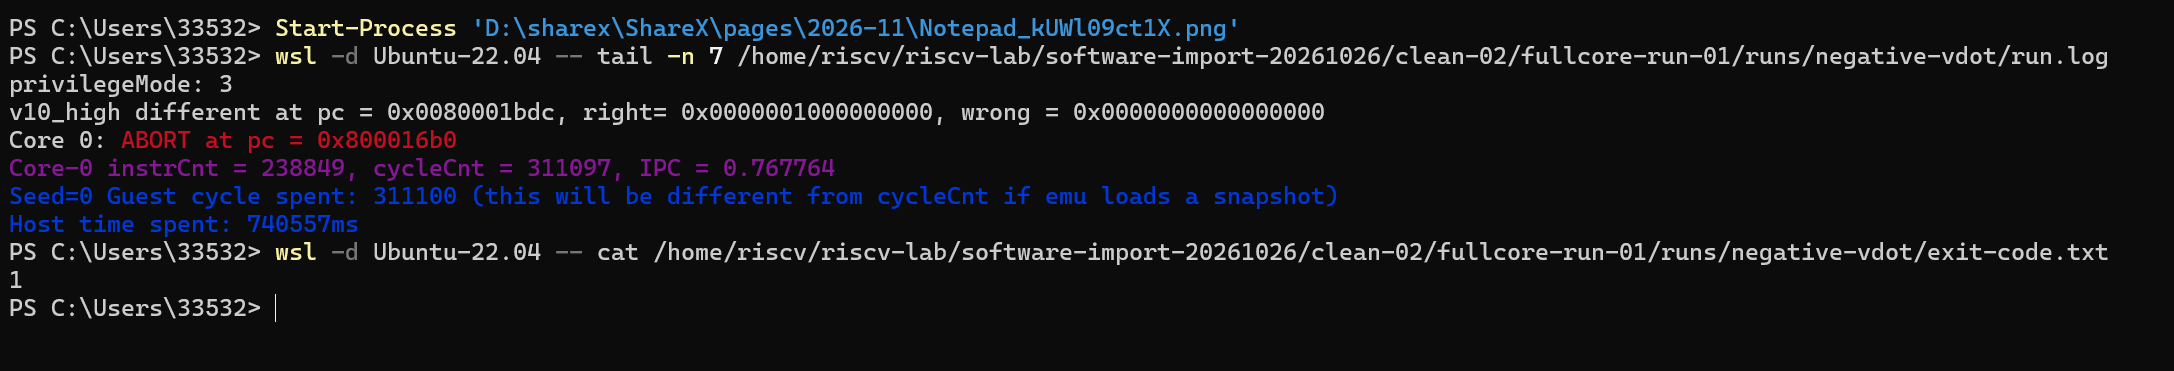
\includegraphics[width=\linewidth,height=4.5cm,keepaspectratio]{figures/source-screenshots/S3-03-01-bit100-rejection.png}
\par\medskip
\textbf{（b）恢复正常参考模型：15项检查通过}\par\smallskip
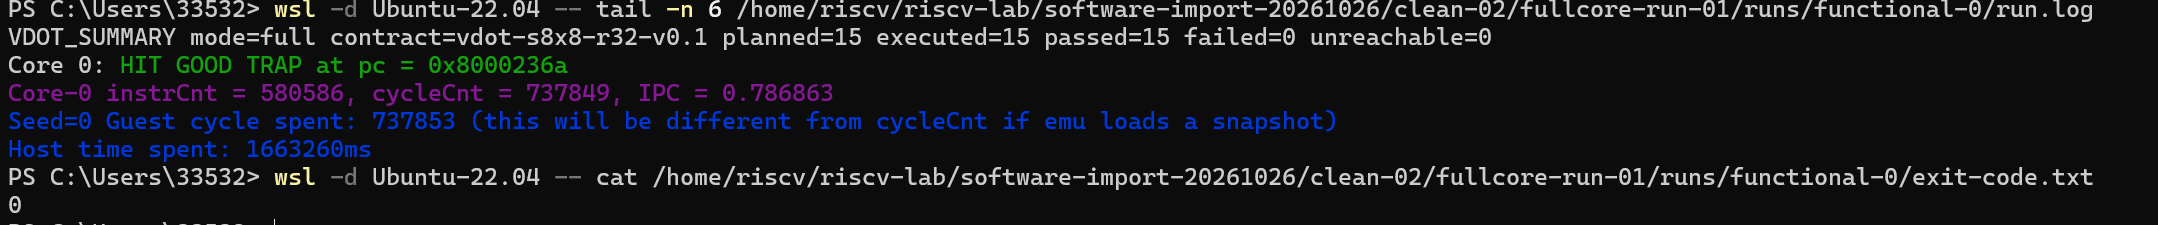
\includegraphics[width=\linewidth,height=4.5cm,keepaspectratio]{figures/source-screenshots/S3-03-02-normal-recovery.png}
\captionof{figure}{高位错误检出与正常参考模型恢复的原始日志}\label{fig:S3-03}
\raggedright\footnotesize
负控日志显示\texttt{v10\_high different}、\texttt{ABORT}和退出码1；差异PC为\texttt{0x80001bdc}，ABORT报告PC为\texttt{0x800016b0}。其中\texttt{right/wrong}是比较器两侧标签，本例的扰动由参考端注入。正常日志显示15项全部通过、\texttt{HIT GOOD TRAP}和退出码0。原记录分别为clean-02的\texttt{negative-vdot}与\texttt{functional-0}；截图及对应运行索引随源包保存。\par
\end{minipage}\end{center}
\end{landscape}
